\documentclass[10pt] {article}
\usepackage[portuguese]{babel}
\usepackage[utf8]{inputenc}
\usepackage{graphicx}

\begin{document}

\title{Relatório Trabalho Prático C \\ $\small{Grupo 13}$}
\author{João Costa \and Leandro Salgado \and Martinho Aragão}

\maketitle

%--------------------------------
% Group Members
%--------------------------------

\begin{flushleft}
João Costa A70563 \\
FOTO
\end{flushleft}

\begin{flushleft}
Leandro Salgado A70949 \\
FOTO
\end{flushleft}

\begin{flushleft}
Martinho Aragão AXXXX \\
FOTO
\end{flushleft}

\newpage

\tableofcontents

\newpage

\section{Módulos}
Na seguinte seção aprasentam-se desenhos comentados das estruturas de dados,
todos os typedef e a documentação da API comentada, função a função.

%------------------------
%	Clients
%------------------------

\subsection{Catálogo Clientes}
\par Esta subsecção trata da API do catálogo de clientes e da sua implementação.

\subsubsection{Estrutura de Dados}
\par
Para guardar os clientes lidos a partir do ficheiro resolvemos usar uma Trie pois apesar de
necessitar de mais instruções a procura é igualmente rápida. A seguir fica um exemplo da Trie implementada, 
cada nodo contêm um caracter e apontadores para próximo, anterior, pai e filhos.

\begin{figure}[ht!]
\centering
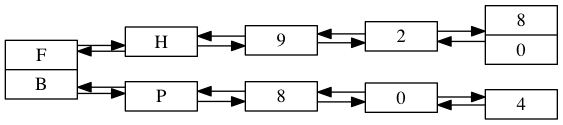
\includegraphics[width=70mm, height=20mm]{trie.png}
\caption{Trie com os clientes FH928, FH920 e BP804}
\end{figure}

\subsubsection{Definições de dados (Typedef)}
\emph{typedef struct node * ClientsCat;} - Catálogo de Clientes
\par Este typedef é a única informação que o utilizador têm relativamente à implementação de dados, não tendo 
acesso ao ficheiro .c dos clientes não consegue conhecer a verdadeira implementação da estrutura \textbf{node}. 
Deste modo garantimos o encapsulamento de dados e a única forma do utilizador interagir com o catálogo de 
clientes será através da API;

\subsubsection{Funções API}

% initClients
\noindent\textbf{ClientsCat initClients()}
\par Inicializa a estrutura do catálogo de clientes.

% insertClient
\noindent\textbf{ClientsCat insertClient (ClientsCat cat, char * client)}
\par Insere um dado client, o argumento \emph{client}, na estrutura de clientes, argumento \emph{cat}.
\par Se a estrutura não tiver sido inicializada ou o cliente não existir a função retornou o valor \emph{NULL},
caso contrário devolve o valor cat, isto permite que duas variáveis trabalhem na mesma estrutura. \\

% searchClient
\noindent \textbf {Bool searchClient (char * client)}
\par Verifica se um cliente, o argumento \emph{client}, existe no catálogo de clientes devolvendo true se existir e 
false caso contrário.

% removeClient
\noindent \textbf{ClientsCat removeClient(ClientsCat cat, char * client)}
\par Remove um cliente, o argumento \emph{client}, de um dado catálogo de clientes, o argumento \emph{cat}.
\par A função retorna \emph{NULL} caso a estrutura não tenha sido inicializada e
retorna a própria estrutura caso contrário. \\

% searchClients
\noindent \textbf{StrList searchClients (ClientsCat cat, char init)}
\par Cria lista com todos os clientes cujo código comece por uma certa letra, o argumento \emph{init}, e que
estejam presentes no catálogo, \emph{cat}, passado como argumento.

% numOfClients
\noindent \textbf{int numOfClients (ClientsCat cat)}
\par Calcula o número de clientes presentes no catálogo, \emph{cat}, fornecido como argumento.

% deleteCat
\noindent \textbf{ClientsCat deleteCat (ClientsCat cat)}
\par Liberta a memória ocupada pelo catálogo de clientes fornecido como argumento, \emph{cat}.
\par A função retorna NULL se a libertação de memória for bem sucedida. \\

% validateClient
\noindent \textbf{Bool validateClient (char * client)}
\par Verifica se um dado cliente, o argumento \emph{client}, é válido. Um cliente é válido se os dois primeiros
caracteres forem duas letras maiúsculas e os restantes três caracteres forem números.
\par A função retorn \emph{true} se o cliente for válido e \emph{false} se não o for.

%------------------------
%	Sales
%------------------------
\subsection{Módulos Compras}

\subsubsection{Estrutura de Dados}
\indent\par Para o Módulo de compras decidimos criar duas estruturas diferentes, apesar de isto significar um maior 
tempo  de inicialização significa também um ganho a nível de rapidez de algumas das queries.
 \par Para ambas as estruturas usamos arvóres AVL, mas numa das arvóres os nodos contêm um código de cliente 
 e um array de 12, meses, apontadores para árvores AVL em que os nodos contêm o código de cliente e a 
 quantidade comprada.
 
\begin{figure}[ht!]
\centering
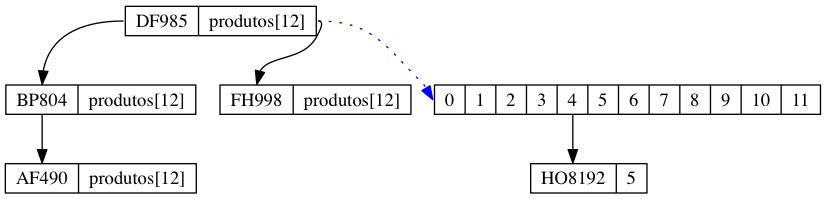
\includegraphics[width=120mm]{avl_salesc.png}
\caption{AVL com clientes, o cliente DF985 comprou 5 unidades do produto HO8192 em Maio}
\end{figure}

\par Na segunda árvore os nodos contêm o código de produtos, a quantidade comprada, o número de clientes que 
 comprou o dado produto e um apontador para uma AVL com os clientes que compraram esse produto e se a 
 compra foi compra normal ou em promoção.

\begin{figure}[ht!]
\centering
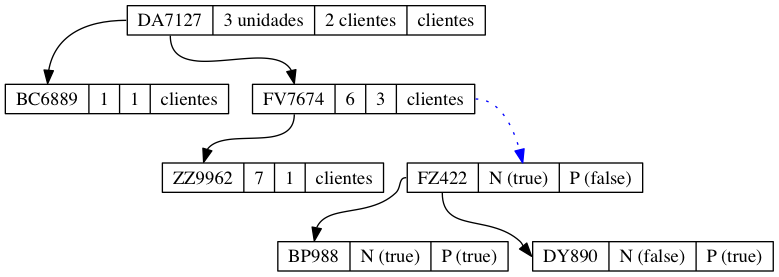
\includegraphics[width=100mm]{avl_salesp.png}
\caption{AVL com produtos, os clientes FZ422, BP988 e DY890 compraram o produto FV7674}
\end{figure}
 
 \subsubsection{Definições de Dados (Typedef)}
 \emph{typedef struct clientNode * SalesC;} - AVL organizada por código de cliente
 \emph{typedef struct productNode * SalesP;} - AVL organizada por código de produto
 \par O utilizador apenas tem acesso a estes dois \emph{typedef} e portanto não tem ideia como está definida a 
 estrutura \textbf{clientNode} e \textbf{productNode}, assim sendo, a única maneira de interagir com o módulo de 
 compras é através das funções disponibilizadas na API.
 
 \subsubsection{API AVL de Clientes}
 % initSales
\noindent \textbf {SalesC InitSales ()}
\par Inicializa a AVL organizada por código de clientes, devolvendo o nodo do tipo \emph{SalesC}.

% insertClientSC
\noindent \textbf {SalesC insertClientSC (SalesC sales, char * client)}
\par Insere um cliente, argumento \emph{client}, na AVL, devolvendo a AVL, é necessário guardar este valor
pois a árvore pode sofrer rotações e não guardando o valor provocará erros em futuras utilizações das funções. \\

%removeClientSC
\noindent \textbf {SalesC removeClientSC (SalesC sales, char * client)}
\par Remove um cliente, argumento \emph{client}, da AVL, argumento \emph{sales}. A função retorna a nova AVL 
sem o nodo de cliente que foi especificado. \\

%insertProductSC
\noindent \textbf {SalesC insertProductSC (SalesC sales, char * client, \\ char * product, int month, int quant)}
\par Insere um produto, \emph{product}, como comprado pelo cliente, \emph{client}, num dado mês, \emph{month}, 
guardando também a quantidade comprada. Se o produto já existir a quantidade é atualizada. \\

%yearlyClients
\noindent \textbf {StrList yearlyClients (SalesC sales, StrList list)}
\par Cria uma lista com os códigos de clientes, presentes em \emph{sales}, que compraram produtos todos os 
meses do ano, guardando numa lista passada como argumento, \emph{list}. \\

%clientMonthlySales
\noindent \textbf {ProductsN clientMonthlySales (SalesC sales, char * client)}
\par Martinho faz esta sff xD. \\

%productsOnMonth
\noindent \textbf {StrList productsOnMonth (SalesC sales, char * client, int month)}
\par Cria uma lista com os produtos comprados por um dado cliente, \emph{client}, num dado mês, \emph{month}, 
caso o cliente esteja presente em \emph{sales}. \\

%topProducts
\noindent \textbf {StrList topProducts (SalesC sales, char * client)}
\par Cria uma lista com os três produtos mais comprados por um dado cliente, \emph{client}, caso esse cliente 
esteja presente em \emph{sales}. \\

%clientMonthlyPurchases
\noindent \textbf {ClientsMonth clientsMonthlyPurchases (SalesC sales)}
\par Outra para ti Martinho, sou mesmo simpático!. \\

%freeSales
\noindent \textbf {void freeSales (SalesC sales)}
\par Apaga a AVL passada como argumento \emph{sales}, libertando toda a memória usada pela mesma. \\

 \subsubsection{API AVL de Produtos}
 % initSalesP
\noindent \textbf {SalesP InitSalesP ()}
\par Inicializa a AVL organizada por código de produtos, devolvendo o nodo do tipo \emph{SalesC}.

\newpage
% insertProductSP
\noindent \textbf {SalesP insertProductSP (SalesP sales, char * product, int quant)}
\par Insere um produto, argumento \emph{product}, na AVL, e uma determinada quantidade \emph{quant}, 
devolvendo a AVL, é necessário guardar este valor pois a árvore pode sofrer rotações e não guardando o valor 
provocará erros em futuras utilizações das funções. Caso o produto exista na AVL a sua quantidade é atualizada.\\

% insertClientSP
\noindent \textbf {SalesP insertClientSP (SalesP sales, char * product, char * client, char type)}
\par Insere um cliente, \emph{client}, na AVL de clientes que compraram o produto, \emph{product}, guardando 
também informação sobre se a compra foi normal, \emph{type} com valor 0, ou compra em promoção, 
\emph{type} com valor 1.\\

% clientsThatBought
\noindent \textbf {StrList clientsThatBought (SalesP sales, char * product)}
\par Cria uma lista com os clientes que compraram um determinado produto, \emph{product}, caso este exista em
 \emph{sales}.\\
 
% topNProducts
\noindent \textbf {topNP topNProducts (SalesP sales, int n)}
\par Devolve uma variável do tipo \emph{topNP} com códigos de produtos, quantidades compradas e número de 
clientes que compraram os produtos, para os \emph{n} produtos mais comprados durante o ano. O utilizador tem 
acesso a definição desta estrutura caso queira usar só uma parte das informações mas esta estrutura apenas 
contêm dados obtidos à partir do módulo de compras. \\

% freeSalesP
\noindent \textbf {void freeSalesP (SalesP sales)}
\par Apaga toda AVL \emph{sales} libertando assim a memória utilizada por este módulo de compras.\\

% UI 
\section{Interface Utilizador}
\par Para ser possível realizar as queries foi necessário criar um menu inicial que não é mais que uma lista 
com opções numeradas e cada opção tem a sua descrição, a partir deste menu inicial o utilizador apenas 
tem que introduzir o número da opção que deseja aceder.
\par Para algumas das queries listas de \emph{Strings} têm de ser apresentadas, essas listas podem variar 
muito  em tamanho e então era necessário uma maneira de as apresentar no ecrã, sem sacrificar a leitura das 
mesmas. 
\par Para apresentar as listas foi criado uma estrutura \emph{StrList} que contêm um array de {* char} e um campo 
com o número de \emph{Strings} guardadas. Decidimos mostrar 20 linhas e 3 colunas de \emph{Strings}, 
dando um total de 60 \emph{Strings} no ecrã ao mesmo tempo, este número faz com que seja fácil visualizar a lista 
quando o terminal ocupa 1/4 do ecrã. As \emph{Strings} são então dividas por páginas e o número de página 
atual e o número total de páginas é apresentado no ecrã.
\par Foi também criado um menu quer permite ao utilizador navegar nas páginas, especificando se quer ir para a 
próxima página, para a página anterior ,para uma página especifica ou então voltar ao menu inicial.
\par Quando o utilizador decide voltar ao menu a função `displayList' liberta todo o espaço em memória utilizado 
pela lista que está a apresentar libertando todas as \emph{Strings} alocadas na lista e no fim libertando a propria 
estrutura.
\par Também há queries que requerem a apresentação de tabelas, para cada uma dessas queries existe uma 
função especializada que trata de apresentar a tabela no terminal do utilizador, contudo a navegação na é 
igual relativamente às listas, os dados são dividos em páginas e as opções de navegação são as mesmas. O único 
aspeto diferente é a apresentação em que cada dado é apresentado na sua própria linha e apenas são 
apresentados 20 resultados de cada vez.

\newpage
\section{Makefile e Gráfico de Dependências}
\indent\par De seguida é apresentada a Makefile, e o gráfico de dependências gerado a partir da Makefile.
\begin{figure}[ht!]
\centering
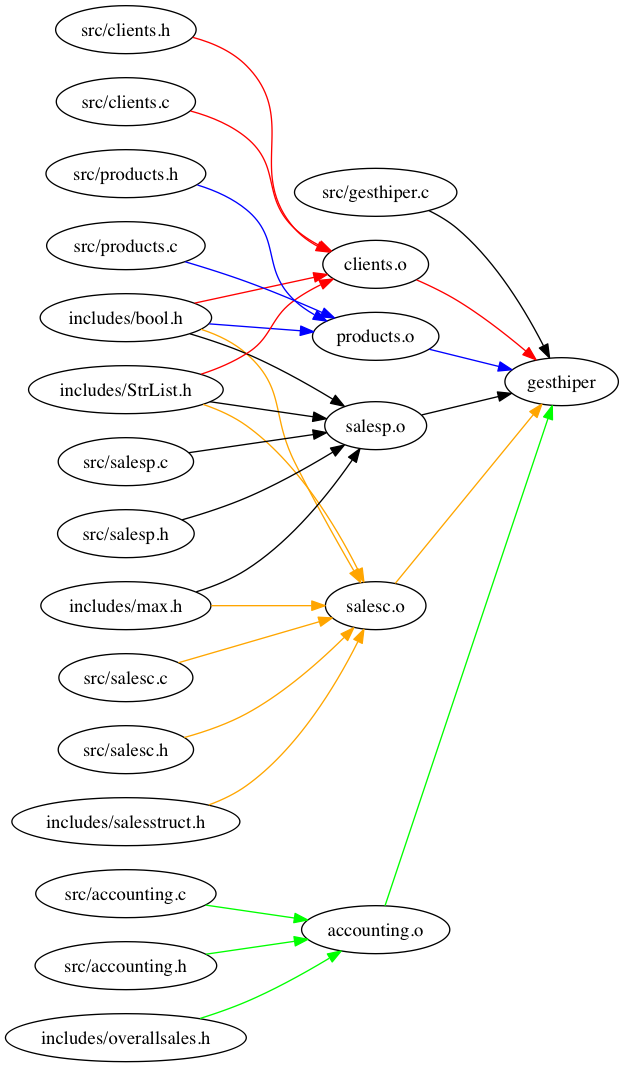
\includegraphics[height=120mm, width=80mm]{dep_graph.png}
\caption{Gráfico de dependências, gerado a partir da Makefile}
\end{figure}
\par O gráfico foi gerado a partir da Makefile:
\small\begin{verbatim}
CFLAGS=-Wall -ansi -pedantic -O2

gesthiper: src/gesthiper.c clients.o products.o accounting.o salesc.o salesp.o
  gcc src/gesthiper.c clients.o products.o accounting.o salesc.o salesp.o
  $(CFLAGS) -o gesthiper -lm
  
clients.o: src/clients.c src/clients.h includes/bool.h includes/StrList.h
  gcc src/clients.c -c $(CFLAGS)
  
products.o: src/products.c src/products.h includes/bool.h
  gcc src/products.c -c $(CFLAGS)

accounting.o: src/accounting.c src/accounting.h includes/overallsales.h
  gcc src/accounting.c -c $(CFLAGS)

salesc.o: src/salesc.c src/salesc.h includes/bool.h includes/max.h 
includes/salesstruct.h includes/StrList.h
  gcc src/salesc.c -c $(CFLAGS)  
   
salesp.o: src/salesp.c src/salesp.h includes/bool.h includes/StrList.h
includes/max.h
  gcc src/salesp.c -c $(CFLAGS)
\end{verbatim}

\end{document}